\section[Lokalisierung (Niklas Schäfer)]{Lokalisierung\begin{tiny} (Niklas Schäfer)\end{tiny}}\label{sec:localisation}
\subsection{Einleitung}
Essentiell für die Auswertung eines Erdbebens mit Smartphones ist die Lokalisierung. Empfängt der Server Alarme von Smartphones, ist es notwendig, dass er unter anderem auch die Standortdaten von der App geliefert bekommt. Zum einen benötigt man eine Lokalisierung um feststellen zu können wo sich das Beben befindet und zum Anderen muss der Server anhand der Standorte der empfangenen Alarme auswerten können, ob es sich um einen korrekten Alarm oder einen Fehlalarm handelt.
Zum Beispiel ist es möglich, dass das Fahren in einem Bus den Beschleunigungssensor Bewegungen wahrnehmen lässt, die einem Erdbeben ähnlich sind, sodass die App von einem Erdbeben ausgehen muss und einen Alarm an den Server sendet. Da der Server bei Alarmen basierend auf Mehrheitsentscheidung urteilt, könnte es passieren, dass er auf ein Erdbeben schließt, wenn mehrere Personen in einem Bus fahren. Daher muss gewährleistet werden, dass es mindestens einen Alarm gibt, der einen bestimmten Mindestabstand zu den betreffenden anderen Alarmen aufweist.

\subsection{Location Provider des Android-Systems}\label{subsec:locProvider}
Im Android System gibt es drei unterschiedliche Location Provider (Verfahren und Sensoren, die einen Standort bestimmen können), die Positionsdaten eines Android Smartphones liefern können:

\begin{itemize}
     \item PASSIVE
     \item NETWORK
     \item GPS
\end{itemize}

\subsubsection{PASSIVE}
Der Location Provider \textit{PASSIVE} initialisiert keinen Zugriff auf einen der vorhandenen Sensoren des Smartphones. Er nutzt lediglich den zuletzt abgerufenen Standort, der sich noch im Speicher des Android Systems befindet. Das heisst, dass er nur den Standort liefert, der von einer beliebigen anderen App oder dem Android System selbst zu irgendeinem Zeitpunkt über die Location Provider \textit{NETWORK} oder \textit{GPS} abgerufen worden ist. Der Vorteil des \textit{PASSIVE} Providers liegt darin, dass er keinen Sensor abfragen muss, sondern lediglich den Speicher ausliest und daher sehr stromsparend fungiert. Für die Quakedetec App ist er allerdings nicht sinnvoll verwendbar, da mit sehr hoher Wahrscheinlichkeit kein ausreichend aktueller Standort vorhanden ist. Es ist beispielsweise möglich, dass die letzte Sensorabfrage schon sehr lange zurück liegt und der Standort veraltet ist.
Somit wäre eine Erdbebenlokalisierung fehlerhaft.

\subsubsection{NETWORK}
Der Location Provider \textit{NETWORK} findet Positionsdaten mit Hilfe von WLAN Netzwerken und der Mobilfunkzelle (\shorthandoff{"}"Mobilfunkmast"\shorthandon{"}). 
Um über WLAN Netzwerke Geräte lokalisieren zu können, pflegt Google eine Datenbank, die WLAN Netzwerke mit Standortdaten verknüpft.
Anfangs geschah dies mit Hilfe des Google Cars, welches hauptsächlich zur Datenerfassung für Google StreetView in vielen Städten unterwegs war. Hierbei erfasste dieses Fahrzeug neben den Straßenbildern auch WLAN Netze und verknüpfte deren MAC-Adresse mit den GPS Daten des Fahrzeugs.
Natürlich sind solche Daten schnell veraltet, weshalb Google weitherin Android Smartphones nutzt, um die Daten aktuell zu halten und neue WLAN Netze in die Datenbank aufzunehmen.
Android Smartphones übermitteln dabei ihren \textit{GPS} Standort, sobald ein solcher ermittelt wurde, zusammen mit den MAC Ids der sichtbaren WLAN Netzwerke in ihrer Umgebung an Google. Dabei wird auch die Signalstärke der WLAN Netzwerke berücksichtigt, um den Standort des WLAN Netzwerks noch genauer ermitteln zu können.
Um einen Standort über den \textit{NETWORK} Provider abzurufen, sendet das Smartphone einen \textit{Request} an Google. In diesem \textit{Request} sind ebenfalls die MAC Ids und Signalstärken der gerade sichtbaren WLAN Netze enthalten. Auch hier werden diese Daten und nicht nur das verbundene WLAN benötigt, um den Standort weiter präzisieren zu können. Würde man nur das verbundene WLAN übermitteln, könnte nur der Standort des einzelnen WLAN Netzes zur Ermittlung des Standorts verwendet werden. Hat dieses WLAN eine hohe Signalstärke, sodass es in einem Radius von mehreren hundert Metern empfangbar ist, wäre der Standort auch nur auf mehrere hundert Meter genau, da nicht bestimmt werden kann, wo sich das Gerät in diesem Empfangsbereich befindet. Bezieht man aber mehrere WLAN Netzwerke mit ein, kann man durch die Überschneidungen der Netze den Standort wesentlich genauer bestimmen. 

\begin{figure}[H]
	\centering
	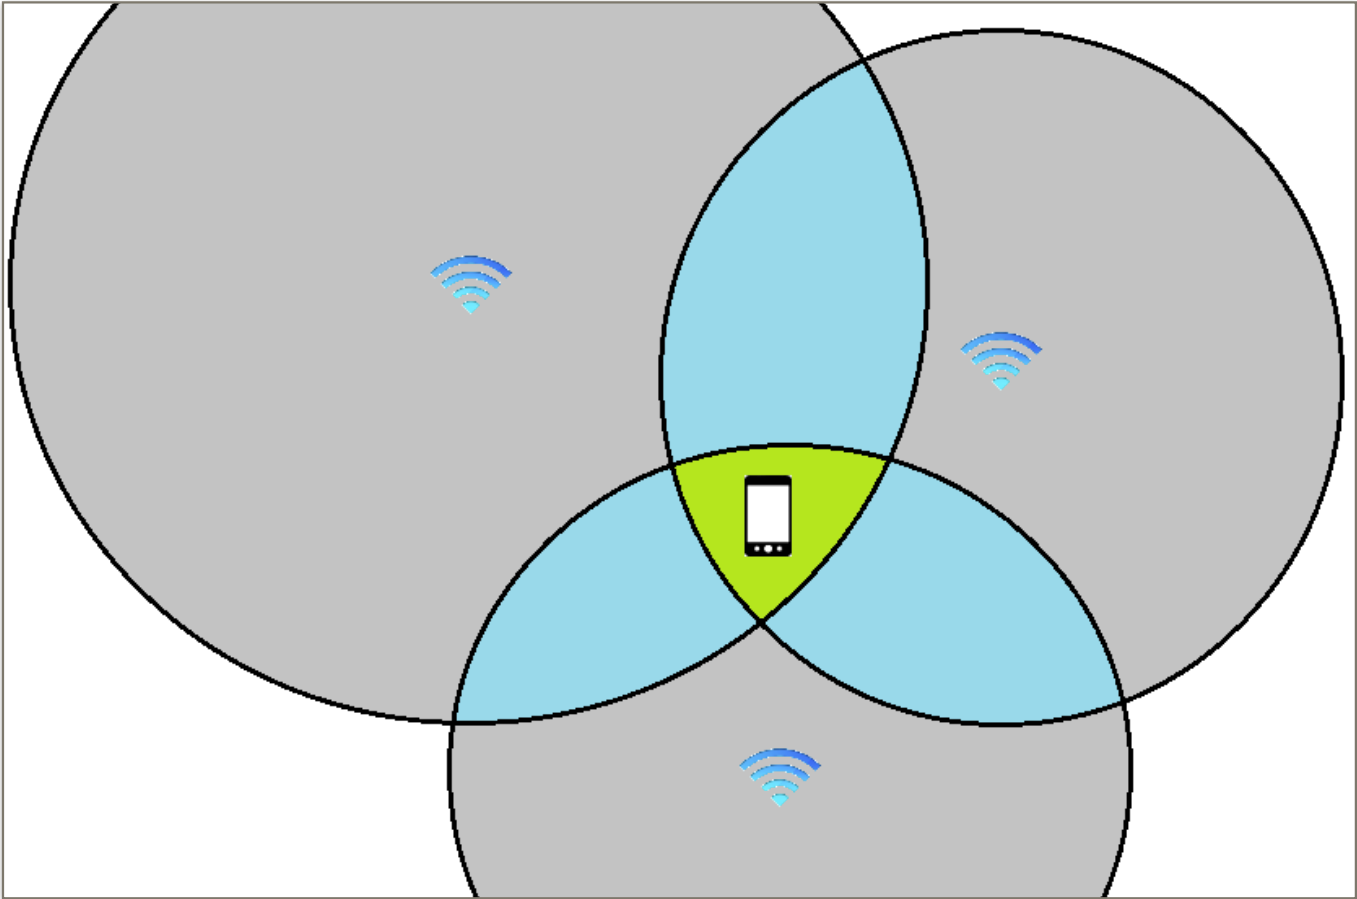
\includegraphics[width=120mm]{/network_provider.png}
	\caption[Lokalisierung: Lokalisierung mit NETWORK Provider]{Lokalisierung mit NETWORK Provider}
	\label{fig:networkProviderfunc}
\end{figure}

In Abbildung \ref{fig:networkProviderfunc} ist die Funktionsweise dieser Lokalisierungstechnik skizzenhaft dargestellt. Ist am Standort allerdings nur ein WLAN Netzwerk sichtbar/verfügbar, bezieht auch hier Google die Signalstärke mit ein, wodurch auch in diesem Fall die Genauigkeit weiter verbessert werden kann.
Wurde der Request vom Smartphone an den Google Server übergeben, werden anhand der gesendeten MAC IDs die verfügbaren Standorte der umgebenen WLAN Netze aus der Google Datenbank entnommen. Daraufhin wird ein Standort mit der beschriebenen Funktionsweise ermittelt (Überschneidungen) und an das Smartphone zurückgesendet. Die Antwort vom Google Server beinhaltet den Längen- und Breitengrad, die Genauigkeit des gelieferten Standorts und einen Zeitstempel. Die Genauigkeit dieses Verfahrens liegt erfahrungsgemäß bei 15-100m.

\begin{figure}[H]
\centering
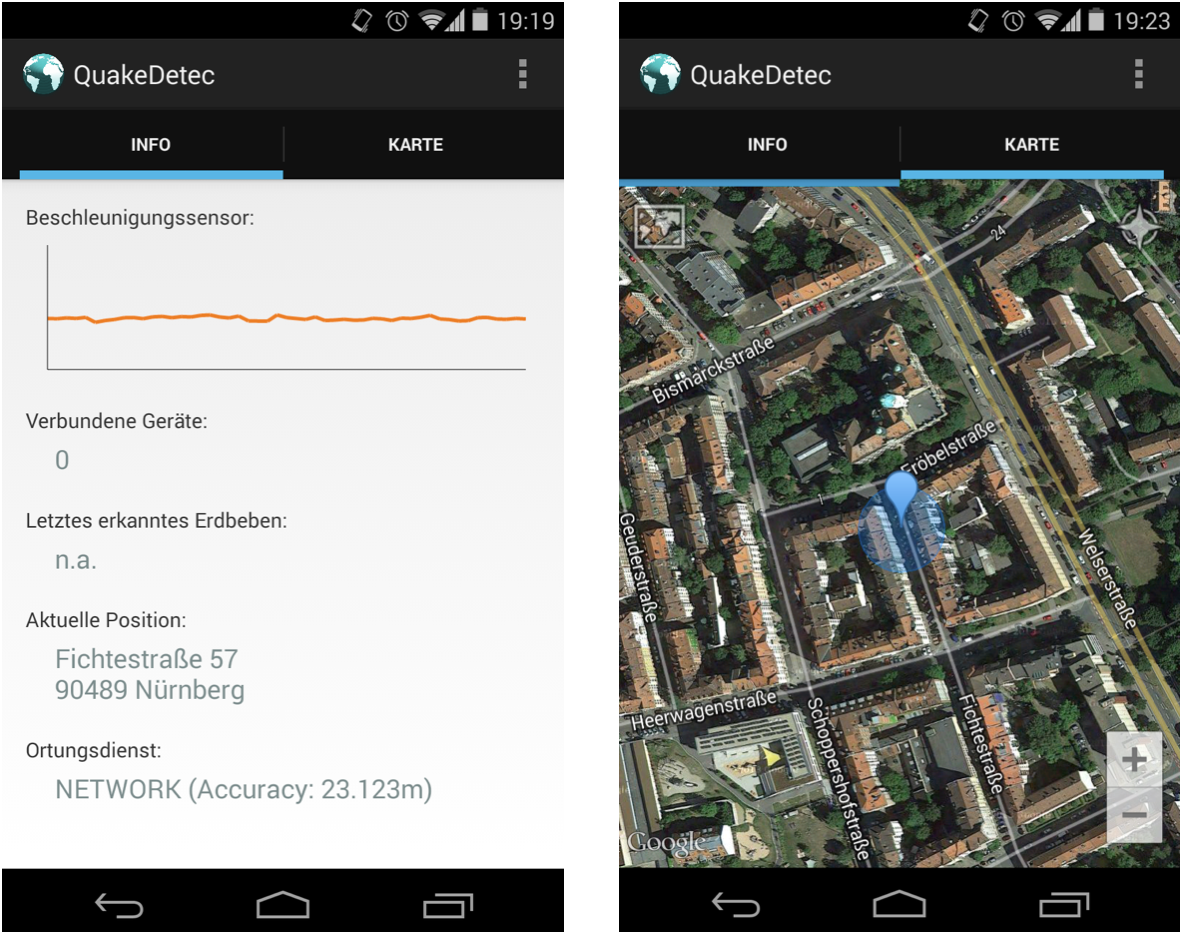
\includegraphics[width=\textwidth]{/network_provider_gui.png}
\caption[Lokalisierung: User Interface bei Nutzung des NETWORK Providers]{User Interface bei Nutzung des NETWORK Providers}
\label{fig:networkProviderGui}
\end{figure}

Sollten keine WLAN Netzwerke verfügbar oder das WLAN des Smartphones deaktiviert sein, nutzt der \textit{NETWORK} Provider die Mobilfunkzellen zur Ortsbestimmung. Dies funktioniert im Grunde nach einem ähnlichen Prinzip, wie die Lokalisierung über WLAN Netze, allerdings werden hierbei keine Überschneidungen mehrerer Mobilfunkzellen berücksichtigt. Google ist der Standort des Mobilfunkmasts ebenfalls bekannt. Um aber auch bei diesem Verfahren mit Überschneidungen arbeiten zu können, müsste das sogenannte Timing-Advance Verfahren verwendet werden. Bei diesem Verfahren wird der Standort ermittelt, indem Signallaufzeiten zum verbundenen Mobilfunkmast gemessen werden. Wird nur die Signallaufzeit zu einem Mast berechnet, kann nur bestimmt werden, welchen Abstand das Gerät zum Mobilfunkmast hat. Um den Standort mit Hilfe von Signallaufzeiten genauer zu bestimmen, ist es notwendig die Signallaufzeit zu mindestens einem weiteren Mobilfunkmast zu messen.

\begin{figure}[H]
\centering
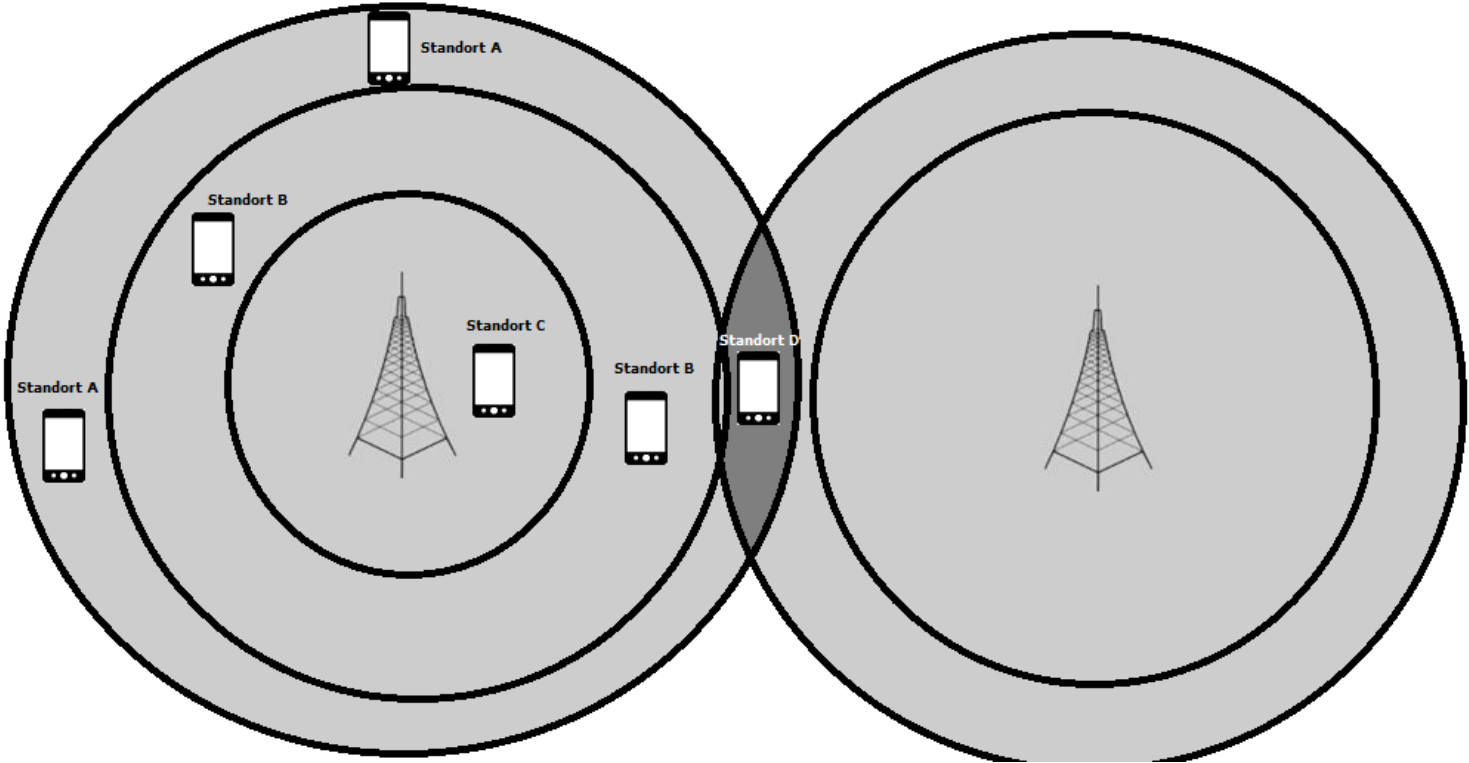
\includegraphics[width=120mm]{/network_provider_timing_advance.png}
\caption[Lokalisierung: Timing-Advance Verfahren]{Timing-Advance Verfahren}
\label{fig:networkProviderTimingAdvance}
\end{figure}


\begin{wrapfigure}{r}{43mm}
\centering
   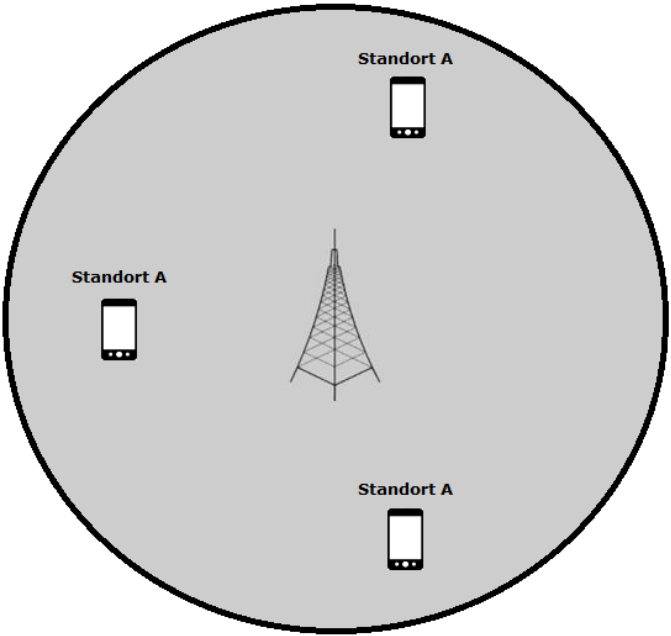
\includegraphics[width=43mm]{/network_provider_praxis.png} 
   \vspace{-5mm}
   \caption[Lokalisierung: NETWORK Provider in der Praxis]{Praxis}
   \vspace{-5mm}
\end{wrapfigure}
Somit gibt es zwei Radien, die sich schneiden und es kann relativ genau ein Standort ermittelt werden. 
Dieses Verfahren findet allerdings kaum Verwendung, da das Gerät dazu gezwungen werden muss die Verbindung zwischen  mehreren Mobilfunkzellen zu wechseln um in jeder Zelle die Signallaufzeit zu messen. Dieser Vorgang führt schnell zu einem hohen Energieverbrauch. Somit wird in der Praxis eine Lokalisierung nur mit Hilfe einer einzigen Mobilfunkzelle durchgeführt. 

Eine Mobilfunkzelle hat eine vielfach höhere Signalreichweite als ein WLAN Netzwerk. In Städten liegt man hier zwar nur bei wenigen hundert Metern, auf dem Land hingegen bei mehreren Kilometern. Somit erhält man in der Stadt meist noch Standortdaten, die auf wenige hundert Meter genau sind, auf dem Land liegt man allerdings meist bei 2 bis 4 Kilometer.

\subsubsection{Global Positioning System}
Mittlerweile besitzt fast jedes aktuelle Android Smartphone einen \textit{GPS} Empfänger. 
Das \textit{Global Positioning System} wurde vom amerikanischen Verteigungsministerium entwickelt. Es besteht aus 30 Satelliten, welche die Erde umkreisen und Nachrichten aussenden, die zur Positionsbestimmung eines Empfängers dienen. Das \textit{Global Positioning System} ist vom Prinzip her der Positionsbestimmung über Mobilfunkzellen im Timing-Advance Modus ähnlich, allerdings im dreidimensionalen Raum. 
Ein Satellit sendet eine Nachricht mit seiner Position und einem Zeitstempel kontinuierlich aus.
Ein \textit{GPS} Empfänger kann aus der Versandzeit einer Nachricht die Signallaufzeit bestimmen (aktuelle Zeit - Versandzeit = Signallaufzeit). Aufgrund der Signallaufzeit kann somit bestimmt werden, in welchem Abstand sich der Empfänger zum Satelliten befindet. 
\begin{wrapfigure}{r}{55mm}
\centering
   \begin{center}
   	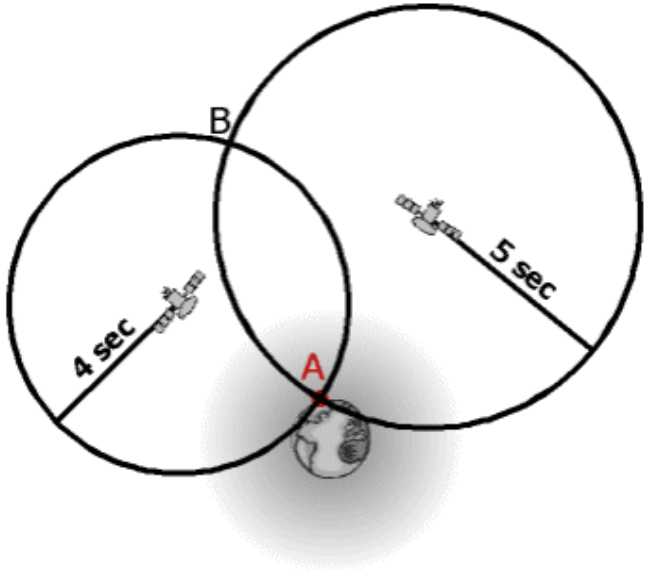
\includegraphics[width=55mm]{/gps_two_satellites.png} 
   \end{center}
   \caption[Lokalisierung: GPS 2 Satelliten]{GPS 2 Satelliten}
   \label{fig:gpsTwoSatellites}
\end{wrapfigure}
Ein einziger Satellit würde zu einer genauen Positionsbestimmung nicht ausreichen, da man nur die Entfernung zu diesem einen Satelliten kennt. Werden aber mehrere Satelliten genutzt, können die Überschneidungen der Radien verwendet werden, um die Position sehr genau zu bestimmen. Mit zwei Satelliten kann theoretisch in einer zweidimensionalen Welt schon eine Position genau bestimmt werden. In Abbildung \ref{fig:gpsTwoSatellites} ist ein Beispiel mit zwei Satelliten zu sehen. Bei der Verwendung von zwei Satelliten gibt es zwei Radien, die sich in zwei Punkten schneiden. Da aber einer dieser Punkte weit im Weltall liegt, kann schnell daraus geschlossen werden, dass nur der andere Punkt Relevant und somit der gesuchte Standort ist. In einer zweidimensionalen Ebene wird in der Realität allerdings noch ein dritter Satellit benötigt, um das sogenannte \textit{Uhrenproblem} zu lösen. Die Satellitenuhren laufen zwar dank Atomuhren absolut genau und synchron, ein \textit{GPS} Empfänger tut dies allerdings nicht. Dadurch würden die Signallaufzeiten bei zwei Satelliten ungenau berechnet werden. 

Mit der Hilfe eines dritten Satellitens kann dieses Problem gelöst werden. 
\begin{wrapfigure}{l}{48mm}
	\centering
	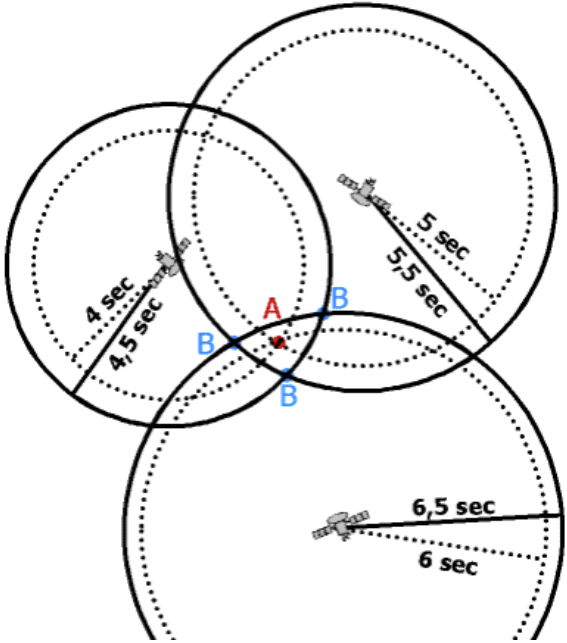
\includegraphics[width=48mm]{/gps_three_satellites.png}
	\caption[Lokalisierung: GPS 3 Satelliten]{GPS 3 Satellites}
	\label{fig:gpsThreeSatellites}
\end{wrapfigure}
Abbildung \ref{fig:gpsThreeSatellites} verdeutlicht die Funktionsweise. Unter der Annahme, dass die Empfängeruhr 0,5s vorgeht, bekommt man Radien die aufgrund der falsch laufenden Empfängeruhr größer ausfallen (durchgezogene Linien/Kreise). In Wirklichkeit fallen diese aber kleiner aus (gepunktete Linien/Kreise). Bei zwei Radien sind bei diesem Szenario zwei Schnittpunkte vorhanden, die eine falsche Position angeben würden, ohne dass es eine Möglichkeit gäbe den Fehler zu erkennen. Wird allerdings ein dritter Satellit zur Bestimmung herangezogen, gibt es bei einer falschen Berechnung aufgrund des Uhrenproblems keinen Schnittpunkt aller drei Radien. In diesem Fall verändert der \textit{GPS} Empfänger seine Uhrzeit so lange, bis sich alle drei Radien in einem Punkt schneiden. Somit wird die Uhrzeit des \textit{GPS} Empfängers mit der Uhrzeit der Satelliten synchronisiert. Der Schnittpunkt aller drei Radien ist dann die exakte Position.
Zur Realisierung dieses Systems und zur genauen Bestimmung der Position in der Realität, also in einer dreidimensionalen Welt, wird noch ein vierter Satellit verwendet. Dies ist notwendig, da in der hier beschriebenen Funktionsweise von einem zweidimensionalen Modell ausgegangen wird. Es kann zwar auch mit diesem Modell die Position in der Realität bestimmt werden, allerdings wird dabei davon ausgegangen, dass sich die zu bestimmende Position auf Meereshöhe befindet. Somit wäre eine Positionsbestimmung falsch, sobald sich der Empfänger über (bzw. unter) dem Meerespiegel befindet.
Bei der dreidimensionalen Positionsbestimmung wird dieses Problem mit einem vierten Satelliten gelöst. Mit diesem ist es auch möglich, die Höhe des Empfängers zu bestimmen. Allerdings soll hier nicht weiter darauf eingangen werden. Dazu der Verweis auf weitere Informationsquellen.

\subsection{Positionsbestimmung in Android}\label{subsec:posInAndroid}

Wie schon in Kapitel~\ref{subsec:locProvider} beschrieben, bietet das Android System drei Möglichkeiten um den Standort zu bestimmen. Um unter Android diese Möglichkeiten zu nutzen, bietet die Android API die drei Location Provider \textit{PASSIVE}, \textit{NETWORK} und \textit{GPS}.
Um einer App den Zugriff auf diese Provider zu gewähren, muss der Zugriff erstmal beim Nutzer erfragt werden. Um diese Berechtigung vor der Installation beim Nutzer einzuholen, muss die folgende Codezeile im Android-Manifest hinzugefügt werden:

\begin{lstlisting}[caption={App Permissions},label=lst:locationPermission]
<manifest ... >
    <uses-permission android:name="android.permission.ACCESS_FINE_LOCATION" />
    ...
</manifest>
\end{lstlisting}

Möchte ein Nutzer die App nun installieren, wird er zuerst gefragt, ob er der App den Zugriff auf die Standortdaten seines Geräts gewähren möchte. Es ist zwingend erfordlich, dass die Abfrage akzeptiert wird, ansonsten wird die App nicht installiert.

\begin{figure}[H]
	\centering
	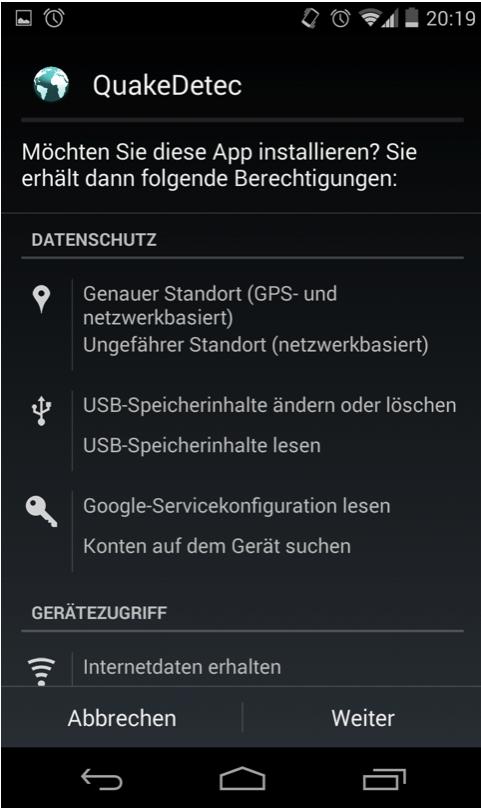
\includegraphics[width=40mm]{/app_permissions.png}
	\caption[Lokalisierung: App Permissions]{App Permissions}
	\label{fig:appPermissions}
\end{figure}

Um in der App auf die Location Provider zugreifen zu können, wird eine Instanz des Android \textit{LocationManagers} benötigt. Mit diesem ist es möglich auf die Location Services zuzugreifen und eine Standortbestimmung auszulösen.

Eine Instanz des LocationManagers erlangt man durch folgende Codezeile:

\begin{lstlisting}[caption={LocationManager Instanz},label=lst:locationManagerInstance, basicstyle=\footnotesize]
// Acquire a reference to the system Location Manager
LocationManager locationManager = (LocationManager) this.getSystemService(Context.LOCATION_SERVICE);
\end{lstlisting}

Außerdem sind LocationListener notwendig, welche beschreiben, wie auf bestimmte Ereignisse der Location Services reagiert werden soll.

Es gibt vier Ereignisse auf die reagiert werden kann:
\begin{itemize}
     \item Neuer Standort
     \item Provider aktiviert
     \item Provider deaktiviert
     \item Status der Provider hat sich geändert
\end{itemize}
Die entsprechenden Methoden des Listeners sind:
\begin{itemize}
     \item \textit{onLocationChanged(Location location)}
     \item \textit{onProviderEnabled(String provider)}
     \item \textit{onProviderDisabled(String provider)}
     \item \textit{onStatusChanged(String provider, int status, Bundle extras)}
\end{itemize}
Hat beispielsweise ein Location Provider einen neuen Standort ermittelt, wird die \textit{onLocationChanged} Methode aufgerufen, der ein \textit{Location} Objekt übergeben wird. In diesem Objekt ist der Längen- und Breitengrad, die Genauigkeit des Standortes in Metern, der Location Provider, der den Standort ermittelte, und ein Zeitstempel enthalten. 
\\
Wird ein Location Provider (z.B. \textit{GPS}) im System deaktiviert, wird die \textit{onProviderDisabled} (bzw. wenn aktiviert \textit{onProviderEnabled}) Methode mit dem Providernamen als Parameter aufgerufen und man kann dementsprechend in der App darauf reagieren. 

\newpage
Das vierte Ereignis auf das reagiert werden kann, ist eine Statusänderung eines Location Providers. Wenn ein Provider aus irgendeinem Grund nicht verfügbar war und wieder verfügbar wird, wird \textit{onStatusChanged} aufgerufen.

\begin{lstlisting}[caption={LocationListener},label=lst:locationListener]
// Define a listener that responds to location updates
LocationListener locationListener = new LocationListener() {
    public void onLocationChanged(Location location) {
      // Called when a new location is found by the network location provider.
      makeUseOfNewLocation(location);
    }
    public void onStatusChanged(String provider, int status, Bundle extras) {}
    public void onProviderEnabled(String provider) {}
    public void onProviderDisabled(String provider) {}
  };
\end{lstlisting}

Um Standortdaten abzufragen, gibt es zwei Möglichkeiten. 
Eine besteht aus der kontinuierlichen Reaktion auf Standortänderungen. Das heißt, dass Standortänderungen zu jedem Zeitpunkt wahrgenommen werden.

\begin{lstlisting}[caption={requestLocationUpdates},label=lst:requestLocationUpdates, basicstyle=\small]
locationManager.requestLocationUpdates(LocationManager.NETWORK_PROVIDER, time, distance, locationListener);
\end{lstlisting}

Dieser Methode wird unter anderem der \textit{Location Provider} und der entsprechende \textit{LocationListener} übergeben. Ein weiterer Parameter steht für die Zeit, die vergangen sein muss, bis wieder ein neuer Standort zurückgegeben wird. Gibt man zum Beispiel 10 Minuten an, wird für 10 Minuten kein neuer Standort zurückgegeben. 
Der letzte verbleibende Parameter steht für die Distanz, die überbrückt worden sein muss, bis ein neuer Standort zurückgegeben wird. Setzt man diesen Parameter zum Beispiel auf 100m, wird ein neu erkannter Standort nur zurückgegeben, wenn die Entfernung zwischen diesem und dem alten mindestens 100m beträgt. 
\\
\\
Eine andere Möglichkeit einen Standort zu ermitteln, ist ein einmaliger Abruf des aktuellen Standorts.
\begin{lstlisting}[caption={requestSingleUpdate},label=lst:requestSingleUpdate, basicstyle=\small]
locationManager.requestSingleUpdate(LocationManager.NETWORK_PROVIDER, locationListener, looper);
\end{lstlisting}

Dieser Methode wird ebenfalls der \textit{LocationListener} und der gewünschte \textit{Location Provider} übergeben. Zusätzlich wird bei dieser Methode noch ein Looper Objekt benötigt, welches eine Messageschleife für Threads bereitstellt.
Diese Methode aktiviert den gewünschten \textit{Location Provider} und wartet, bis ein Standort von diesem zurückgegeben wurde. Danach wird der \textit{Location Provider} wieder deaktiviert und es werden keine neuen Standorte mehr ermittelt.

\subsection{Umsetzung der Quakedetec App}
\subsubsection{Erste Umsetzung und Probleme}
Anfangs wurde die App mit der \textit{requestLocationUpdates} Methode (siehe Kapitel \ref{subsec:posInAndroid}) und dem \textit{NETWORK} und \textit{GPS} Provider umgesetzt. Es wurden beide Sensoren kontinuierlich abgefragt und der genauere

\begin{wrapfigure}{r}{50mm}
\centering
   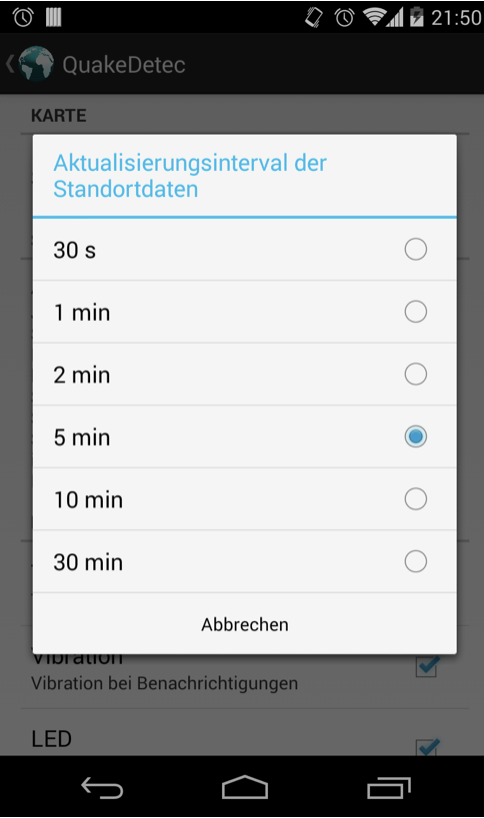
\includegraphics[width=50mm]{/locationupdates_interval_ui.png} 
   \caption[Lokalisierung: Update Interval]{Update Interval}
\end{wrapfigure}

und aktuellere Standort der beiden Location Provider wurde verwendet. Da man im Falle eines Erdbebens den Standort des Geräts benötigt um die Erdbebenposition zu bestimmen, erachteten wir es als sinnvoll, den Standort kontinuierlich zu bestimmen. Diese Möglichkeit bot die \textit{requestLocationUpdates} Methode. Allerdings fiel schnell auf, dass der Akkuverbrauch mit dieser Lösung sehr hoch und somit inakzeptabel war. Um dieses Problem zu lösen, fügten wir in der App die Einstellung für ein Aktualisierungsintervall hinzu. Über diese Einstellung stellten wir eine Möglichkeit zur Verfügung, in der \textit{requestLocationUpdates} Methode den Parameter für die Zeit zu setzen (in Kapitel \ref{subsec:posInAndroid} beschrieben). Das bot dem Nutzer die Möglichkeit das Zeitintervall zu bestimmen, welches vergangen sein muss bis ein neuer Standort zurückgegeben wird. Zum Zeitpunkt der Implementierung war uns nicht bewusst, dass diese Umsetzung keine Auswirkung auf den hohen Akkuverbrauch haben wird. Denn nicht wie zuerst angenommen, sinkt zwischen dem Intervall der Energieverbrauch der Sensoren, sondern er bleibt identisch, da die Sensoren trotz des Zeitintervalls durchgehend aktiv bleiben.
Das heißt, dass der Standort trotz des Intervalls durchgehend ermittelt wird, nur dass der Standort ausschließlich nach Verstreichen des Intervalls zurückgegeben wird.
Als uns dies bewusst wurde, stellten wir die Lokalisierung auf Singleupdates um (\textit{requestSingleUpdate}, siehe Kapitel \ref{subsec:posInAndroid}). Diese Singleupdates wurden mit Hilfe eines Timer Threads, welcher in einem Hintergrundservice lief, ausgeführt. Nun wurde das Interval dieses Timer Threads über die Einstellung in der App geregelt. Somit war dies nun ein reales Intervall in dem die Sensoren deaktiviert werden. 
Das brachte zwar eine Verbesserung der Akkuleistung, aber der Verbrauch war selbst bei einem 10 Minuten Intervall noch zu groß. Außerdem war diese Umsetzung nicht vereinbar mit der benötigten Aktualität der Standortdaten. Denn letztendlich kann sich ein Nutzer innerhalb von 10 Minuten schon an einem ganz anderen Standort befinden. Wurde beispielsweise eine Standortaktualisierung 9 Minuten vor einem Erdbebenalarm ausgelöst und der Benutzer war in dieser Zeit in Bewegung, sind die an den Server übermittelten Standortdaten nicht mehr aktuell und können stark von der tatsächlichen Position abweichen. Somit war diese Lösung ebenfalls inaktzeptabel und die Implementierung musste überdacht werden.

\subsubsection{Finale Umsetzung}
Das Problem des hohen Akkuverbrauchs konnte schnell ausfindig gemacht werden. GPS ist zwar mit einer Genauigkeit von drei Metern sehr präzise, aber der GPS Sensor hat einen sehr hohen Akkuverbrauch. Außerdem besteht ein weiteres Problem von \textit{GPS} darin, dass eine Sichtverbindung zu Satelliten bestehen muss, was zur Folge, dass eine Positionsbestimmung innerhalb von Gebäuden nicht möglich. Und schließlich werden sich viele Nutzer überwiegend innerhalb von Gebäuden aufhalten.
Somit entschlossen wir uns, überwiegend auf GPS zu verzichten und primär auf den \textit{NETWORK} Provider zurückzugreifen. Dieser bietet den Vorteil, dass er sehr stromsparend arbeitet und innerhalb von Gebäuden ebenfalls nutzbar ist. In Städten besitzt dieser Provider durch die hohe WLAN- und Funkzellendichte eine hohe Genauigkeit. Bei Tests in Nürnberg lag die Genauigkeit zwischen 20-50m.
\begin{wrapfigure}{r}{60mm}
\centering
   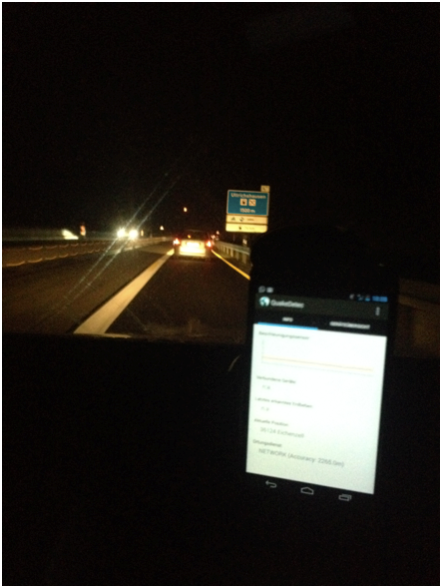
\includegraphics[width=60mm]{/test_autobahn.png} 
   \caption[Lokalisierung: Test auf der Autobahn]{Test auf der Autobahn}
\end{wrapfigure}
Leider hat er den Nachteil, dass er auf dem Land sehr ungenau werden kann, da hier oft keine WLAN Netze und nur sehr wenige Mobilfunkzellen vorhanden sind. Bei durchgeführten Tests beispielsweise in einem ländlichen Raum in der Nähe Bad Hersfelds und auf Autobahnen, lagen die schlechtesten Werte bei 3400m. Laut Informationen des Geoforschungszentrums Potsdam, die wir durch E-Mail Kontakt erhielten, ist dieser Wert kein sehr großes Problem bei der Erdbebenerkennung, allerdings kommt hierbei zum tragen, dass zum Teil mehrere Benutzer in einem Senderadius eines Mobilfunkmasts genau den gleichen Standort zugeordnet bekommen können, und zwar den des Funkmasts. Das führt zu der Problematik, dass wir bei einer Erdbebenauswertung auf dem Server nicht feststellen können, ob sich die Nutzer genau am selben Standort oder weit voneinander entfernt befinden. Bei der Erdbebenauswertung mit Hilfe einer Mehrheitsentscheidung muss allerdings ausgeschlossen werden, dass sich die Nutzer nicht am gleichen Ort (z.B. in einem Radius von 100m) befinden. Denn sollten z.B. mehrere Nutzer in einem Bus unterwegs sein und aufgrund erdbebenähnlicher Bewegungen des Busses einen Erdbebenalarm an den Server senden, würde bei der Auswertung ein Erdbeben festgestellt werden. Um diesen Fall auszuschließen, wird bei der Erdbebenauswertung immer überprüft, ob mindestens ein Gerät der alarmauslösenden Geräte mindestens 100m von den anderen entfernt befindet. Das kann im schlechtesten Fall im ländlichen Raum bedeuten, dass ein Gerät mindestens soweit von den anderen entfernt sein muss, sodass es mit einer anderen Mobilfunkzelle verbunden ist. Das heißt bei dem von uns am schlechtest gemessenen Wert von 3400m, muss eines von den alarmauslösenden Geräten mindestens 3401m vom Funkmast entfernt sein, damit es einen anderen Standort zugewiesen bekommt und man sich bei der Auswertung sicher sein kann, dass sich die Geräte nicht am selben Standort befinden. Um zu gewährleisten, dass die Ungenauigkeit nicht zu groß wird, wurde die Lokalisierung so implementiert, dass bei einer Genauigkeit höher als 3500m der GPS Sensor aktiviert wird und über diesen ein genauer Standort abgerufen wird.
Das heißt zusammenfassend, dass die App im seltenen worst-case Szenario nur Erdbeben erkennt, die weiter strahlen als 3500m, sodass Geräte in einem Radius, der größer als 3500m ist, das Beben noch wahrnehmen können.
Die Implementierung auf diese Weise stellte den besten Kompromiss zwischen Akkuverbrauch und Genauigkeit dar, da der GPS Sensor somit nur sehr selten verwendet wird. Ebenfalls wurde Rücksprache mit dem Geoforschungszentrum Potsdam gehalten und wo uns mitgeteilt wurde, dass Erdbeben, die weniger als 3500m strahlen, so schwach sind, dass von ihnen keine Gefahr ausgeht. 
\par\bigskip
\begin{quote}
\shorthandoff{"}"Ihre Frage war, ob für ein Beben, das nur in einem Umkreis von 3,5km gespürt werden kann, eine Frühwarnung ausgesprochen werden sollte. Unserer Meinung nach kann man darauf verzichten, denn es kann sich aufgrund des eingeschränkten Bereiches (gefühlt in kleiner 3,5km) nur um ein kleines Beben handeln, das kein Schadenspotenzial besitzt."\shorthandon{"}\newline
(Claus Milkereit, GFZ Potsdam)
\end{quote}
\newpage
\begin{wrapfigure}{r}{50mm}
	\centering
	\label{notification_localizer_app}{
    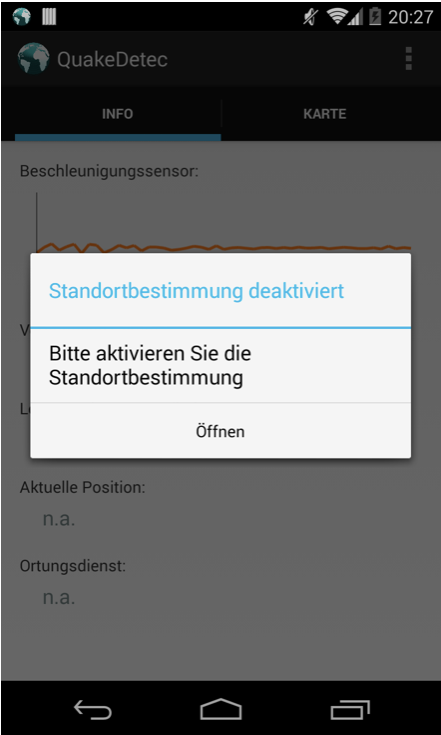
\includegraphics[width=49mm]{/notification_localizer_app.png}}
    \vspace*{-2mm}
    \caption[Lokalisierung: Notification in der App]{Notifications}
	\vspace*{5mm}
	\label{notification_localizer_statusbar}{
    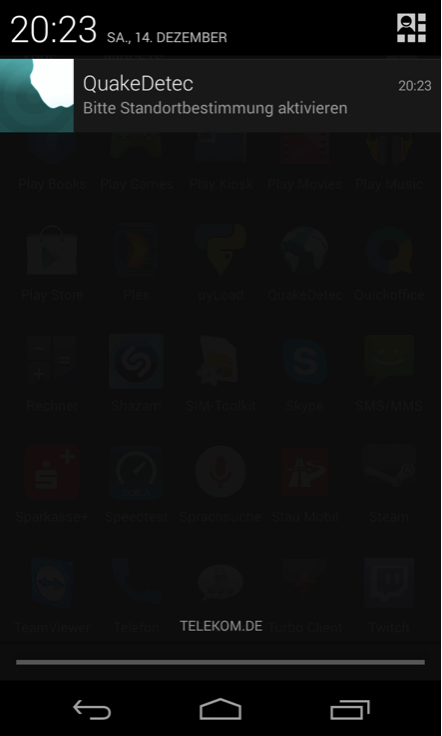
\includegraphics[width=49mm]{/notification_localizer_statusbar.png}}
    \vspace*{-2mm}
    \caption[Lokalisierung: Notification bei geschlossener App]{Notifications}
    \vspace*{-10mm}
\end{wrapfigure}
Da die App abhängig von den Standortdaten ist und ohne Lokalisierung nutzlos ist, prüft die App, ob zumindest eine der beiden Lokalisierungsmethoden (\textit{NETWORK} oder \textit{GPS}) im Android System aktiviert ist. Ist dies nicht der Fall, wird bei geöffneter App ein Popup angezeigt, welches den Nutzer auffordert, die  Lokalisierung zu aktivieren. Tippt der Nutzer auft \shorthandoff{"}"Öffnen"\shorthandon{"}, werden die Android Systemeinstellungen für die Lokalisierung geöffnet. In der App schließt sich das Popup erst, wenn eine der beiden Lokalisierungsmethoden aktiviert wurde. 
\par\bigskip
Läuft die App im Hintergrund und der Nutzer deaktiviert die Lokalisierung, gibt die App eine Android Notification in der Android Statusbar aus. Diese kann vom Nutzer nicht geschlossen werden und schließt sich ebenfalls erst nach der Aktivierung einer Lokalisierungsmethode und kann nicht vom Nutzer geschlossen werden.

\par\bigskip
Um das Problem der Aktualität der Daten zu lösen, wurde die Standortabfrage flexibel gestaltet. Ist die App geöffnet und sichtbar, wird die Standortabfrage in einem Intervall von 30s ausgeführt. Das Intervall ist bei geöffneter App kurz gewählt, damit gewährleistet wird, dass der Nutzer in der Standortanzeige und der Google Map einen relativ aktuellen Standort angezeigt bekommt. Ist die App nicht sichtbar und läuft im Hintergrund, wird eine Standortabfrage in einem Intervall von 10 Minuten ausgeführt. Diese Abfrage ist notwendig, da die App alle 10 Minuten einen Heartbeat mit dem Standort an den Server sendet. Außerdem wird ein Standort abgefragt, sobald ein Erdbeben erkannt wurde und wird mit dem Alarm an den Server gesendet. Da ein Alarm in der App zeitkritisch ist und eine Standortabfrage mit Hilfe des GPS Sensors eine längere Zeit beanspruchen kann, wird zusätzlich in einem Intervall von fünf Minuten eine Standortabfrage unabhängig vom Heartbeat oder Alarm ausgeführt. Somit kann sichergestellt werden, dass ein Standort der mit einem Alarm gesendet wird, nicht älter als fünf Minuten ist, falls die Standortabfrage unmittelbar vor dem Alarm zuviel Zeit in Anspruch nimmt und nicht auf diese gewartet werden kann.

\subsubsection{Klassendiagramm Localizer}
\begin{figure}[H]
	\centering
	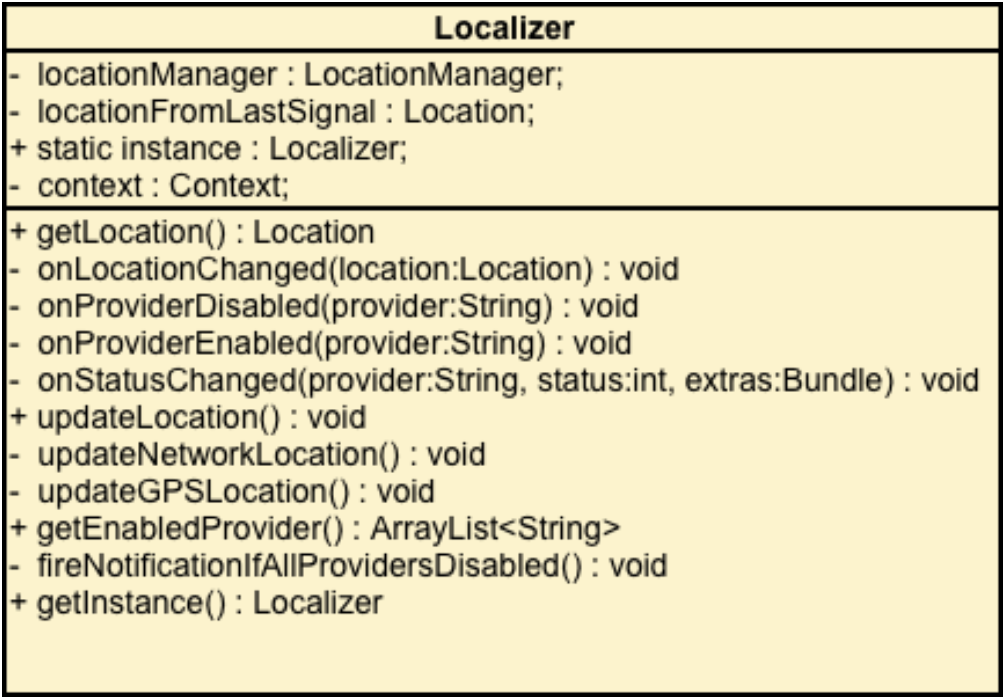
\includegraphics[width=\textwidth]{/localizer_class.png}
	\caption{Lokalisierung: Localizer}
	\label{fig:localizerClass}
\end{figure}